\chapter{Photogrammetry - II}

With transformations we want to transfer coordinates from various systems to another. From the world coordinate system, to the camera coordinate system, to the image coordinate system.

In the pipeline of transforming coordinates, there are extrinsics and intrinsics. The extrinsics describe the pose of the camera in the world. Intrinsic parameters describe the mapping of the scene in front of the camera to the final image. 

\textbf{Key Convention Point}

In a regular pinhole camera, the image is formed BEHIND the camera center. This is obviously how physics works but for the near entirety of this field, we will consider the image formed in front of the camera center. This is purely to make representation and math simpler. Obviously, this doesn't change anything or invalidate "normal" math as the figures will actually be congruent.

\section{Camera Intrinsics and Extrinsics}

Extrinsic parameters describe the pose of the camera in the world. On the other hand, intrinsics describe the mapping of the scene imaged to the the image taken.

\textbf{Extrinsics}

There are 6 parameters to represent the extrinsics - 3 for position + 3 for direction. The translation between origin of world and camera center represents the transformation $X_O = [X_0, Y_0, Z_0]^T$. Then, there is a rotation matrix $R$ that represents the direction of the camera. 

\textbf{Intrinsics}

The process of projecting points from the camera to the image and to the sensor requires intrinsics. We come across more of this later.

\subsection{Calibration}

Quite often, we read that a camera has to be calibrated prior to use. When calibrating a camera, we are trying to estimate some parameters - intrinsics. These parameters are critical to processing our image such as correcting lens distortion, determining the camera's location and so on.

\begin{figure}[h]
    \centering
    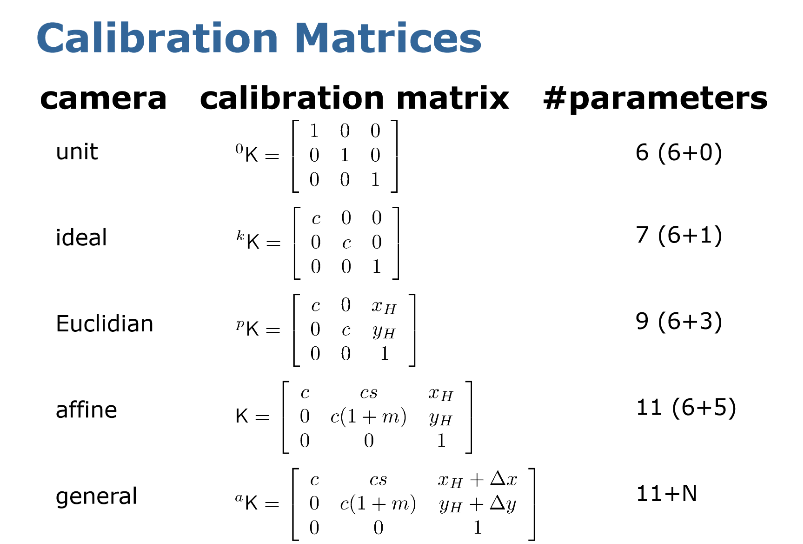
\includegraphics[width=12cm]{img/calibration-matrices.png}
    \caption{Calibration Matrices}
    \label{fig:calibration}
\end{figure}

The image \ref{fig:calibration} is useful to see what various calibration matrices we have. Some of these will be introduced later. Note that a scaled version of these projection matrices will also project to the same point - due to the nature of the homogeneous coordinates.

\section{Projection Matrix}

On multiplying the projection matrix with the camera coordinates, we obtain the projected image coordinates. This projection matrix is a camera instrisic that is defined with the focal length values. 

I didn't write this section until after the next lecture. Look at the section on Camera Modelling in chapter 13 to read more about how projections are represented.

\section{Transformations}

Transformations include shearing, rotation, scaling, each of which can be represented using a single matrix.

\subsection{2D Rotations}

\begin{equation}
    R = \begin{bmatrix}
    \cos\theta & -\sin\theta \\
    \sin\theta & \cos\theta 
    \end{bmatrix}
\end{equation}

This transformation is orthonomal such that $R^{-1}=R^T$. Here, the column vector correspond to the new axes that are formed after rotating that particular vector.

\subsection{3D Rotation}

With 3D rotation, we can rotate the body along any particular axis. So, when we rotate along the $z$ axis for instance, it means that you "fix" the z axis and move the $x$ and $y$ axes. Hence, the $z$ coordinate doesn't change but the X-Y coordinate changes - just as they would in the 2D rotation case. Hence, the rotation matrix is:

\begin{equation}
    R_{z}(\theta) = \begin{bmatrix} 
    \cos\theta & -\sin\theta & 0 \\
    \sin\theta & \cos\theta & 0 \\
    0 & 0 & 1
    \end{bmatrix}
\end{equation}

In general, the matrix can be seen as a table where the column headers are $x, y, z$ of the new frame and the rows are the initial frame. The elements in $j^{th}$ column and $i^{th}$ row is in fact the PROJECTION of the $j^{th}$ point (can be seen as a vector from origin) on the $i^{th}$ axis - always assuming the unit vector (why should we consider scaling here anyway).

Look up the rotations along other axes. We needn't have just rotations along one axis though. But, it is still simple! Let's assume that we have some rotation in mind that is not along a particular axis. We can make the same rotation along one axis and then along another axis. This is hence, a product of two rotations along the axis. We can string together various axis rotations in such a manner to get any general rotations. 

Rotations are always relative to the current frame.

Rotations in real life are quite interesting as often they do not just "rotate" an object, but also change the direction in which a component is pointing at. Imagine a robotic arm that is spray painting. If we didn't consider direction, on rotating the arm, it would paint in a different direction altogether.

\subsection{Scaling}

Scaling is obviously just stretching vectors along a particular direction. For instance, $x'=sx$. This can be represented by a matrix :

\begin{equation}
    \begin{bmatrix}
    x \\
    y\\
    z\\
    \end{bmatrix}' = \begin{bmatrix}
    s & 0 & 0 \\
    0 & u & 0 \\
    0 & 0 & t \\
    \end{bmatrix} \begin{bmatrix}
    x \\
    y\\
    z
    \end{bmatrix}
\end{equation}

This will not change parallelism, ratio of lengths in any direction.

\subsection{Shearing}

With shearing, we are essentially stretching a vector along a certain direction. Note that we are stretching, not displacing. Now, when we are stretching a square on a 2D plane, assume that there is a resulting parallelogram. Clearly, all points in the square were not shifted equally. In fact, the greater the $y$ coordinate, the greater it was shifted on the $x$ axis. This is precesily how we write our shearing matrix:

\begin{equation}
    \begin{bmatrix}
    1 & x_y & x_z \\
    y_x & 1 & y_z \\
    z_x & z_y & 1
    \end{bmatrix}
\end{equation}

\subsection{Reflection}

With reflection, we neflect around a particular axis. Hence, we negate along a particular axis. So the matrix could look like:

\begin{equation}
\begin{bmatrix}
-1 & 0 & 0\\
0 & -1 & 0 \\
0 & 0 & 1
\end{bmatrix}
\end{equation}

\subsection{Translation}

Translation is the only transformation that is represented by a particular vector. But, with homogeneous coordinates we can represent it as a matrix.

\section{Frames}

In a lot of places, we refer to transforming points and frames. It's intuitive to think of frames as the coordinate system. Hence, transformations on our frame shifts our coordinate system. The origin and axes change with the transformations.

\section{Axis-angle representation}

This is a different way to represent rotations using a pair of vector and angles. He did not explore this in more depth, but it helps avoid some problems with other representations. For example [0,0,30] indicates along [0,0,1] axis, rotate by 30 degrees. \textit{I think he said that axis angles are euclidian - this is huge since rotation matrices aren't euclidian!}